\chapter{Analys och diskussion}

Under projektets gång fattades många beslut och det stöttes även på en del
problem. Grunden till dessa beslut och lösningar på problemen diskuteras i
detta kapitel.

\section{Metod}

Här diskuteras utvecklingen av projektet både ur ett tekniskt perspektiv och
ett metodikperspektiv.

\subsection{Systemarkitektur}

I projektets början diskuterades vilka programmeringsspråk och ramverk som
kunde passa. De språk som ansågs vara lämpliga för systemet var Javascript,
Google Dart, Phyton, PHP och Ruby. För- och nackdelar mellan de olika språken
diskuterades. Slutledningen blev att PHP gick bort ganska snabbt på grund av
att det ansågs inte vara det optimala språket då det ansågs onödigt svårarbetat
samt att PHP är inte ett fullständigt objektorienterat språk till skillnad från
Ruby on Rails \cite{shiftdynamic}. Google Dart gick bort på grund av att
gruppen inte hade någon tidigare erfarenhet av språket. Av de kvarstående
språken var det Ruby med ramverket Ruby on Rails som var mest attraktivt
eftersom det redan fanns kompetens om språket och ramverket i gruppen.

Beslutet om att använda Ruby on Rails hade både för och nackdelar. Nackdelarna
var att språket har en hög inlärningströskel. Eftersom det är ett fullständigt
objektorienterat språk kräver det att programmeraren förstår hur alla
\emph{controllers} och \emph{models} fungerar. Som nybörjare var det svårt att
förstå principen för designmönster MVC. Det var också svårt att förstå och
börja använda Rubys syntax i början. Då Ruby är ett så kallat script-språk är
det svårt att applicera kunskaper från högnivåspråk som C++.

En av fördelarna med att använda Ruby on Rails var att små förändringar i koden
kan göra stora förändringar i systemet. Till exempel finns det många
hjälpfunktioner man kan dra nytta av vilket gör att koden kan hållas kort och
koncis. Det går också väldigt lätt att dela upp koden i olika filer vilket gör
att varje fil aldrig innehåller särskilt många rader kod. Dock kan det ta lång
tid att hitta rätt fil när hela projektet har delats in i många små filer om
det inte finns en tydlig struktur och namngivning.

Ytterligare fördelar med att använda ett webbramverk finns och kan
generaliseras med att säga att det är onödigt att uppfinna hjulet på nytt.
Säkerhet, effektivitet och struktur är aspekter som förstärks utav många
ramverk. En mer konkret fördel med Ruby on Rails är modulen
\texttt{ActiveRecord} som alla modeller i systemet ärver av.
\texttt{ActiveRecord} har funktioner för att hantera relationer och frågor mot
databasen.

När Angularjs började användas höjdes svårighetsgraden ytterligare. Efter att
gränssnittet började ta form gick det nästan inte att göra förändringar i
systemet utan att använda Angularjs. Därför blev det en förutsättning att varje
gruppmedlem hade en förståelse för ramverket eftersom samtliga utvecklare
jobbade på hela systemet.

Fördelen med Angularjs är att detta ramverk hanterar datan som ska presenteras
på ett mycket smidigt sätt \cite{angularjs}. Utan att använda ett ramverk som
Angularjs hade det tagit mycket lång tid för webbläsaren att presentera datan
och koden hade blivit väldigt komplicerad och ineffektiv. Nackdelen med
Angularjs var den samma som Ruby on Rails, att det tar tid att förstå och är
svårt att hantera i början.

En annan fördel med Angularjs är dess stöd för så kallade templates och för
dess tvåvägsbindning för variabler \cite{angularjs}. Tvåvägsbindningen gjorde
det enklare att utveckla komponenter som beror på hur användaren interagerar
med textfält eller knappar. Till exempel krävdes det väldigt lite ansträngning
för att uppdatera en rubrik till det som användaren skrev i ett textfält
samtidigt som denne skrev, eller att uppdatera både textfältet och rubriken
samtidigt.

\subsection{Filhantering}

I inledningen av projektet utvecklades systemet endast med tanken att det
skulle vara ett lager ovanpå Dropbox. Då kundens krav förtydligades efter
insikten att Dropbox kräver kostnadsbelagda servertekniker (krypterad och
certifierad anslutning) fyra veckor in i projektet, var gruppen tvungna att
göra en omvändning och prioritera om vad som skulle utföras och i vilket skede.
Istället för att fokusera på enbart Dropbox lades då fokus på Google Drive.
Detta visade sig dock otillräckligt enligt kund på grund av de begränsningar i
lagringsutrymme Google Drive har. Det var först där efter som arbetet med den
lokala filhanteringen inleddes. Det blev då tydligt att gruppen fokuserat på
fel funktionalitet sett till kundens önskemål under flera veckor. Detta misstag
kan ha berott på bristande kundkontakt och teknisk studie. Om en teknisk studie
angående Dropbox och Google Drive hade påbörjats tidigare, hade dessa
implementationer fått lägre prioritet medans lokal lagring hade fått högre
prioritet. På så sätt hade projektets fokus blivit rätt från början.

Ett alternativ som övervägdes för att sköta filhanteringen var Mongodb. Detta är en dokumentdatabas som istället för att lagra tabeller med information lagrar dokument med identifierade nycklar som indexeras av databasen. Mongodb har dessutom stöd för att ha en kolumn med binär fildata och inte bara siffror eller strängar. Denna kolumn med fildata skulle alltså användas för att lagra filerna, snarare än att skriva dem i serverns filsystem. Detta valdes dock bort för att minska insteget till att utveckla systemet samt för att hålla nere antalet mjukvaror som systemet berodde av.

Skapandet av \emph{trigrams} för filer skedde från början vid samma tillfälle
som när en fil skapas i databasen. Detta gjorde så att varje förfrågan
blockerades av systemet för att skapa dessa. När det var många filer som lades
till samtidigt kunde väntetid bli påtaglig för användaren, för att lösa detta
implementerades Delayed Job, en \emph{gem}. Istället för att det skapas direkt
i vid förfrågan sköts skapandet upp och skedde senare i en separat process.
Skillnaden i tid gick från att en förfrågan tog 392 millisekunder till 55
millisekunder vilket ansågs vara en markant förbättring.

\subsection{Taggning och sökning}

För att uppnå en effektiv sökstruktur efter filer i en databas finns det två olika metoder: professionell indexering och folksonomi som tidigare nämnts i kapitel \ref{sec:tags}.

Fördelarna med professionell indexering är att den är mer precis jämfört med
folksonomi eftersom det går att rama in den eftersökta informationen med
huvudkategorier och underkategorier. Det går alltid att ta sig fram i
databasens olika kataloger och till slut hitta den sökta filen. Folksonomi,
till skillnad från professionell indexering, baserar sin sökning på taggar och
på grund av det är det inte säkert att nyckelorden leder rätt. Användare kan ha
olika uppfattning om vad basnivån är på innehållet vilket gör att antingen
onödiga taggar läggs till eller att det finns brist på taggar. Om till exempel
en Javascript-fil ska taggas kan det vara onödigt för en användare att tagga
filen med ``webb'' medan det är nödvändigt för en annan. Därför kan ett
traditionellt klassificeringssystem ge ett bättre resultat eftersom det är helt
opersonligt.

Eftersom systemet främst är till för den enskilde användarens strukturering av
filer för att snabbt kunna finna dem igen är folksonomi att föredra. Ett
kundkrav var dessutom att hierarkin skulle vara platt, vilket professionell
indexering inte uppfyller.

Då det inte finns någon stavningskontroll när taggen skrivs in kan användaren
använda  slanguttryck och dialektala uttryck som kan precisera innehållet.
Fördelen med att låta användaren stava taggarna precis som denne vill är att
det blir lättare att skräddarsy taggarna för användarens egna ändamål. Det är
också mindre kostsamt att använda sig av folksonomi till skillnad från
professionell indexering. Professionell indexering kräver att det finns en noga
genomtänkt katalogstruktur och regler för vart innehållet ska placeras. I ett
taggningssystem krävs det inte alls lika mycket eftertanke från användaren
gällande vilken katalog denne ska börja leta i. Det krävs bara att söka efter
ett någorlunda passande nyckelord.

\subsection{Hantering och strukturering av databaser}

Systemet använder sig idag utav en relationell SQL-databas för dess data;
användare, taggar samt filer lagras som rader i olika tabeller. Ett alternativ
till relationella SQL-databaser av denna typ som övervägdes är så kallade NOSQL-
databaser. Ofta står detta för \emph{Not Only SQL} och är en samlingsterm för
databaser som inte nödvändigtvis är tabellbaserade \cite{nosql}. Exempel på
typer som ingår i denna samling är dokument-baserade databaser (databasen
lagrar indexerade filer) och nyckel-värde-lagringar (data lagras i listor med
nyckelord som används för att komma åt dem). Gemensamt för denna samling
databastyper är att de inte har en fast struktur och undviker relationer till
andra databaser eller uppsättningar \cite{largedata}. Dessa typer av databaser
valdes tidigt bort på grund av dess icke-relationella struktur, samt på grund
av deras mindre utvecklade stöd för användning i en Ruby on Rails-program.

\subsection{Gränssnitt}

Tanken med gränssnittet var att fokusera på filpresentationen. Eftersom alla
filer presenteras i en och samma lista hade systemet blivit för långsamt och
överväldigande om alla filer skulle visas samtidigt. Därför skapades en knapp
för att ladda in fler filer successivt.

Överst i gränssnittet har en huvudmeny fixerats för att användaren snabbt ska
kunna nå funktioner som utloggning, inställningar och filimportering. Det är
funktioner som används ofta och bör vara lättillgängliga. Eftersom varje fil
innehåller så pass mycket metadata som namn, datum, filtyp, \texttt{Identity}
och taggar krävs det att fil-listan breder ut sig över hela skärmen för att
kunna visa denna information. Ändringar av filer i systemet görs med ikonerna
längst ut till höger i listan. I de flesta lagringstjänster kommer användaren
åt dessa funktioner genom att högerklicka på filen. Genom att ha ikonerna
synliga från början blir det färre klick för att utföra dessa operationer.

\begin{Figure}
  % center it!
  \centering
    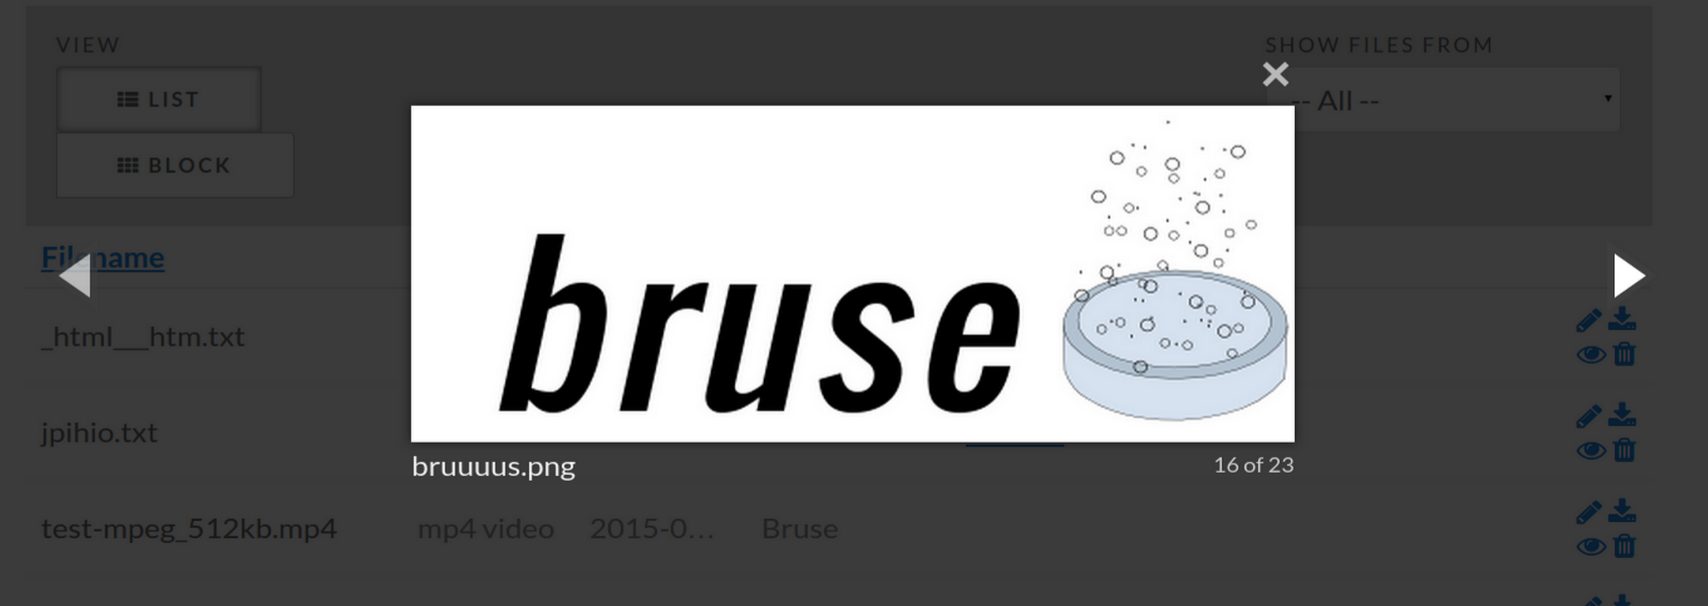
\includegraphics[width=0.9\linewidth]{figures/screenshots/preview.png}
    \captionof{figure}{\emph{Förhandsgranskning av fil.}\label{fig:preview}}
\end{Figure}

Förhandsgranskningen av filer sker genom att filen visas i webbläsaren med
hjälp av en gem som heter Magnific Popup. Magnific Popup gör att filen som ska
förhandsgranskas lägger sig som ett lager över allt annat. Förhandgranskaren
gör det möjligt att bläddra fram och tillbaka mellan alla filer som lagts till
och för att stänga ner förhandsgranskningen är det bara att klicka på det
skuggade området eller på krysset, se figur \ref{fig:preview}. Den här typen av
förhandsgranskning är mycket vanlig bland andra tjänster och är väldigt
praktisk på grund av att piltangenterna går att använda för att bläddra mellan
filerna och att det går snabbt att komma tillbaka till fillistan.

\subsection{Testning}

Under projektets början följdes planen att skriva tester efter varje funktionsimplementering, men vid förändrade förutsättningar i sprint två uppstod problem med testningen. Då användarhanteringen byggdes om med hjälp av tredjepartsbiblioteket Devise förändrades hur sessioner hanterades av systemet och följderna blev att de redan skrivna testerna misslyckades.

Det tog för lång tid att hitta en lösning för hur den nya sessionshanteringen skulle kunna testas. Därför valdes att nedprioritera testning. Tester togs bort och eftersom problemet aldrig löstes försvann testning från arbetsflödet och togs aldrig upp igen. \emph{Build}-servern var kvar under utvecklingen som fortsatt kontroll att inget i systemet kraschar.

Testningen gav en bekräftelse vid kodgranskning att systemet och det nyligen
utvecklade funktionerna inte förstörde något tidigare. Dock krävdes mycket tid
för att få igång många system. Att testa javascript med hjälp av Phantomjs var
viktigt då stora delar av systemet byggdes i Javascript men det tog tid att
installera och implementera. Även \emph{fixtures}, som tas upp i kapitel
\ref{sec:4test}, tog tid att få igång på det sätt som gjorde att systemets
funktionalitet gick att testa.

\subsection{Utvecklingsmetodik}

För att fungera som ett team är det en förutsättning att man fördelar
ansvarsområdena så att alla får en roll i projektet. Enligt Scrum måste det
finnas en scrummästare och en produktägare . Utöver dessa roller utsågs en
testansvarig, dokumetansvarig och kodansvarig. scrummästaren hade lite svårt i
början med att komma in i sin roll och se till att mötena genomfördes enligt
scrumprinciperna men blev bättre efter återkoppling i samband med en
sprintåterblick.

Det uppstod problem vid projektets början på grund av dålig kommunikation inom
gruppen vilket gjorde att två personer började arbeta på samma funktion
samtidigt utan att veta om det. Det hade räckt att bara en person arbetade med
funktionen och låtit den andra arbeta med något annat för att vara effektiva.
Detta problemet togs upp på ett möte och det bestämdes att gruppen skulle prata
mer med varandra och vara mer aktiva på Trello för att samma misstag inte
skulle upprepas.

Arbetsrutinerna var att arbeta cirka tre hela dagar varje vecka, motsvarande
60\% av en arbetsvecka. Hade någon inte möjlighet att närvara under bestämd tid
fick denne ta igen arbetet vid något annat tillfälle. Mycket av tiden gick åt
att sätta sig in i hur teknikerna som användes fungerade. Det ledde till att de
lägre prioriterade kraven inte implementerades som till exempel e-posthantering
och implementationen av Mongodb.

Fördelen med Scrum var att gruppen ständigt uppdaterade varandra om vad som var
gjort och vad som skulle göras. Detta gav utvecklingsteamet en uppfattning om
hur arbetet låg till tidsmässigt. Sprintåterblickar var speciellt bra då
problem som uppstått både inom gruppen och kodmässigt togs upp och kunde
åtgärdas.

Ibland var det svårt att tidsuppskatta en uppgift från ett scenario vilket
ledde till att vissa scenarier aldrig hann slutföras innan sprintavslutningen.
Helst ska alla scenarier i sprintbackloggen vara avklarade innan sprinten
avslutas för att hålla sig till tidsplanen. Om så inte var fallet löstes det
genom att skicka över ej avslutade scenario till nästa sprint. I sprint ett var
det särskilt många scenarior som inte blev slutförda vilket berodde på att
inlärningen för nya verktyg tog tid och att rutinerna för kodgranskningen gick
långsamt i början.

Valet att avsluta sprint två tidigare än vad som var planerat visade sig vara
ett bra beslut. Efter mötet med kunden fanns det ny funktionalitet som skulle
implementeras vilket ledde till stora förändringar jämfört med vad som var
planerat för denna sprint. Det krävdes diskussioner kring hur den lokala
fillagringen skulle fungera, men till slut hade alla i gruppen en ganska klar
bild hur detta skulle lösas vilket underlättade för nästa sprintplanering.

Under arbetet jobbade gruppen utan att ha några milstolpar för projektet. Det
sattes inte upp mål för när vissa funktioner skulle vara klara annat än att
varje scenario hörde till en sprint. Om gruppen hade satt upp tydligare mål för
varje sprint och större, sprintöverskridande mål, hade det med stor sannolikhet
varit lättare att hålla tidsmålen. Om detta även hade kombinerats med fler
kundmöten hade projektet med stor sannolikhet också blivit mer framgångsrikt.

En förbättringpotential finns också för gruppen då de dagliga scrummötena inte
utnyttjades fullt ut. Dessa mötens fulla potential finns i att det som sägs tas
med under resten av dagen. Med detta menas att varje gruppmedlem måste tänka
efter noggrant kring vad som faktiskt gått bra sedan det senaste mötet, vad som
gått sämre och vad som skall göras den kommande dagen. Dessa möten blev
rutinmässiga istället för eftertänksamma, vilket hämmade syftet med dem.

\subsection{Versionshantering och kodgranskning}

Github har varit till fördel för utvecklarna genom möjligheten till
versionshantering och kodgranskning. Varje utvecklare kunde arbeta på en egen
komponent utan att grunden ändrades. Det här arbetssättet medförde dock att det
ibland blev en konflikt då två utvecklare arbetat inom samma komponent, men i
två olika förgreningar. Detta löstes med att grenarna antingen slogs ihop innan
de sammanfogades med grunden, eller att ena grenen sammanfogades med grunden
först.

Arbete genom förgrening kan också bli problematisk då en gren bygger på en
annan. Detta gav mestadels problem för kodgranskningen, eftersom det var svårt
att sätta sig in i den påbyggda grenen utan att ha granskat grenen den bygger
på. Detta löstes genom att teamet avvaktade med den senare grenen.

Ett annat problem har varit när en gren har blivit för stor och därmed blivit
svårgranskad på grund av dess omfattning. Det här har utvecklingsteamet försökt
undvika genom att hålla förändringarna små  samt kontinuerligt och ofta
sammanfoga varje förgrening med grunden.

\subsection{Källkritik}

Mycket av informationen angående programmeringen har hämtats från olika
webbsidor. Både Ruby on Rails och Angularjs har väldokumenterade kodexempel på
sina hemsidor som pedagogiskt förklarar grundprinciperna. Det fanns även
dokumentation för alla \emph{gems} som användes, dock med varierande kvalitet.
Denna dokumentation fanns dels tillgänglig via Github och dels från diverse
internetguider och artiklar. Trots att det fanns bra dokumentation var det inte
alltid tillräckligt med hjälp. Det behövdes ofta göras eftersökningar på fler
kodexempel för att kunna använda till exempel en \emph{gem} eller Google Drives
API (Application Programming Interface). Kodexempel och diskussioner som inte
kommer direkt ifrån bibliotekens utgivare bör användas mer kritiskt. I vissa
fall var information från forum där vem som helst kunnat föreslå lösningar den
enda hjälpen som gick att få tag på.

Inledningsvis var internetguider i form av filmer till stor nytta, för att öka
förståelsen för Ruby on Rails. Ett exempel på en sida som användes var Railscast
\footnote{railscasts.com} som var till hjälp eftersom sidan har ett brett
filmarkiv som behandlar både triviala och avancerade implementationer i Ruby on
Rails. Problemet med internetguider är att programmeringsspråken uppdateras
relativt ofta vilket gör att guiderna blir föråldrade och ibland odugliga trots
att de kan behandla rätt ämne.

\section{Resultat}

Nedan diskuteras hur väl det färdiga systemet levde upp till de förväntningar
som inledningsvis fanns på det. Vad kunde gjorts annorlunda vad hade detta
kunnat leda till?

\subsection{Filhantering}

Som nämnts tidigare hade gruppen inledningsvis fel fokus vad gäller
filhantering. Exempelvis kunde mer tid ha lagts på att utveckla den lokala
fillagringen ytterligare. Istället för att skriva direkt till samma server som
sköter systemets logik kunde en annan tjänst använts om mer tid hade funnits.
Några exempel på detta är Mongodb, vilket tas upp i kapitel \ref{sec:local},
eller exempelvis Amazons Simple Storage Service, som är en tjänst för att lagra
stora volymer data i molnet.

Vidare hade systemet kunnat göras effektivare genom att minimera det
lagringsutrymme som krävs utav tjänsten. En metod för detta är att se till att
en fil aldrig lagras av systemet mer än en gång. Säg till exempel att flera
användare lagrar en textfil som innehåller texten ``Hej''. I dagsläget lagrar
systemet en kopia av denna fil för varje användare, istället för att lagra en
gemensam referens till filen för alla. Genom att generera så kallade hashar för
samtliga filer, textsträngar som beror på innehållet i en fil och skapas med
hjälp av matematiska operationer, kan filers likhet konstateras \cite{
datastructures}. Detta skulle kunna användas för att se om användaren laddar
upp en fil som redan har en identisk like i systemet.

En annan aspekt som kunde utvecklats ytterligare är säkerheten kring den lokala
fillagringen. Filerna är idag inte publikt åtkomliga, endast systemet kan läsa
och skriva till dem och de finns inte att komma åt publikt via internet. Vidare
döps filerna om till en slumpad kombination av siffror och bokstäver, vilket
gör dem svårare att identifiera vid ett eventuellt intrång. För att veta vem en
fil tillhör behövs således både databas och fil med andra ord behövs fler
pusselbitar behövs för att få hela bilden. Om någon obehörig person skulle få
tag på en fil fanns det dock inget som hindrade denne person från att öppna den.

\subsection{Tredjepartsverktyg och bibliotek}

Användning av \emph{gems} hjälpte till att öka funktionaliteten i systemet.
Gems till exempel som Devise sparade mycket programmeringsarbete till skillnad
från om funktionaliteten hade skrivits från grunden. Även om det fanns
svårigheten med att hantera vissa tillägg under utvecklandet ansågs det att den
tid som lades på att förstå sig på tillägget var väl värd. Detta eftersom det
var en relativt liten ändring, jämfört med tilläggets storlek och totala
funktion, som behövdes åtgärdas eller justeras.

\subsection{Krav}

Kundens alla krav uppfylldes inte då de prioriterades olika och därmed hann
inte vissa krav bli verklighet. Ett av dessa krav var att kunna spara e-post
och att tagga dessa.

\section{Arbetet i ett vidare sammanhang}

Här diskuteras hur det färdiga systemet ställer sig i relation till omvärlden. Vilka etiska krav ställer systemet på användare och utvecklare?

\subsection{Fildelning}

I dagens elektroniska samhälle är illegal fildelningen ett problem,
upphovsrättsskyddat material delas utan tillstånd från upphovsrättsinnehavaren.
Samtidigt är det svårt att kontrollera illegal fildelning utan att inkräkta på
användarens integritet. Därför är det upp till användaren att inte använda
webbtjänsten till att dela upphovsrättsskyddade filer.  Liknande tjänster som
Dropbox eller Google Drive har större resurser för att motverka att användaren
använder tjänsten på otillåtna sätt jämfört med vad detta system har
\cite{techcrunch}.

\subsubsection{Filhantering}

Det är viktigt att ha en tjänst som hanterar filer på ett säkert sätt så att
obehöriga inte kan få tillgång till dem. Därför är det viktigt som utvecklare
att se till att systemet inte har några säkerhetsbuggar som kan leda till att
känslig information kan nås från obehöriga användare.

\subsubsection{Olagliga filer}

Ansvaret för vad som laddas upp ligger enbart hos användaren. I Sverige är det
olagligt att publicera information som bryter mot: hets mot folkgrupp,
uppvigling, barnpornografi samt olaga våldsskildring \cite{polisen}. Om det
upptäcks att en användare sprider den här typen av information är det ett
lagbrott vilket kommer leda till att polisen får utreda ärendet.

\subsubsection{Personlig integritet}

Då tjänsten är gjord för att kunna spara vilka filer som helst har ägaren utav
servern där systemet körs en skyldighet att låta den informationen som sparas i
databasen vara fortsatt hemlig för utomstående eller andra användare utav
systemet. Koder för att komma åt användares Google Drive- och Dropbox-konton
sparas i databasen. Även om dessa är temporära och databasen är skyddad med
lösenord kan alltid ägaren av servern se innehållet i databasen.
